%!TEX root=kdd15_workshop_main.tex
\section{Evaluation}
We ran our distributed experiments on a subset of the Edison machine at NERSC, featuring 5576 compute nodes with two 12-core Intel ``Ivy Bridge'' processors per node and a Cray Aries interconnect. 

We evaluate \ourmethod by its runtime as well as the quality of the partition that it produces. 

We measure the partition quality by the \textit{fraction of cut edges} $\lambda$.
\begin{align}\lambda = \frac{\text{Number of edges cut by partition}}{\text{Total number of edges}}\end{align} where lower numbers represent a higher degree of locality. We can compare this to our baseline, the expected quality of a random $k-$partition, $\lambda_r = \frac{k-1}{k}$. Any partitioner that produces partitions with $\lambda < \lambda_r$ has improved the parallel locality of the partitions.

\todo{Discuss balance.}

\subsection{Test Graphs}
We discuss our results with both synthetic and real-world graphs. While synthetic graphs make for excellent scalability experiments, demonstration on real-world networks is important to verify that the partitioner works well in practice. 

\subsubsection{Real-world Graphs}
The SNAP dataset is a collection of real-world networks collected by Leskovec and collaborators~\cite{Leskovec-data, snapnets}. 
Many networks in this collection are power-law and scale-free representatives of social networks (such as collaboration networks, citation networks, email networks, and web graphs). We consider these to be excellent representatives of the sorts of data that will continue to increase in size, and have run \ourmethod on a representative selection of graphs, outlined in~\RefTable{tab:rw}.

\begin{table}
\caption{Basic properties of graphs in SNAP data set~\cite{Leskovec-data}, and $\lambda$ for one pass. $\lambda_{r,2}=0.5,\lambda_{r,8}=0.87$}
\rowcolors{2}{blue!05}{blue!15}
\centering
\small
{ \begin{tabular}{ *5r }    \toprule
\emph{Data Set} & $N$ & $nnz$  & $\lambda_{k=2}$ & $\lambda_{k=8}$ \\\midrule
soc-LiveJournal & 4,847,571 & 68,993,773  &0.234& 0.463\\
as-Skitter & 1,696,415 & 22,190,596  & 0.166&0.324\\
cit-Patents & 3,774,768 & 16,518,948  & 0.402&0.726\\
roadNet-CA & 1,971,281 & 5,533,214  & 0.186&0.360\\
web-Google & 916,428 & 5,105,039  &0.189&0.336\\
wiki-Talk & 2,394,385 & 5,021,410 &0.411&0.752\\
amazon0302 & 262,111 & 1,234,877 & 0.202&0.370\\
soc-Slashdot0902 & 82,168 & 948,464  &0.236&0.382\\
ca-AstroPh & 18,772 & 396,160 & 0.232&0.413\\
cit-HepPh & 34,546 & 421,578 & 0.343&0.646\\
email-EuAll & 265,214 & 420,045 & 0.280&0.538\\
Oregon-1 & 11,492 & 46,818  & 0.224&0.406\\
p2p-Gnutella04 & 10,879 & 39,994  & 0.415&0.747\\
 \hline
\end{tabular}\par
}
\label{tab:rw}
\end{table}

\subsubsection{Synthetic Graphs}
For scalability experiments we generated random undirected power-law Kronecker (RMAT) graphs of varying scale in parallel using the Graph500 Reference implementation~\cite{graph500}. Kronecker graphs are commonly used in HPC graph benchmarks and testing, and arbitrarily large instances can be efficiently generated in parallel. The \emph{scale} of an RMAT graph is equal to $\log |V(G)|$, and the edge-factor is the average number of edges per node, which we hold constant at 16. Vertex and edge counts for the scales we experiment on are shown in~\RefTable{tab:rmat}.

\begin{table}
\caption{Edge and vertex counts for generated RMAT graphs of each scale.}
\rowcolors{2}{blue!05}{blue!15}
\centering
\small
{ \begin{tabular}{ l | c | c | c | c | c | c  }    \toprule
\label{table:rmat}
Scale & 26 & 27 & 28 & 29 & 30 & 31 \\ \midrule
|V(G)| & 67M & 134M & 268M & 537M & 1.07B & 2.15B \\%& 4.29B \\
|E(G)| & 1.07B & 2.14B & 4.29B & 8.58B & 17.1B & 34.3B \\%& 68.7B \\
\hline
\end{tabular}\par
}
\label{tab:rmat}
\end{table}

\todo{Discuss the iterative stream figures.}
\RefFigurePair{fig:k2_lambda, fig:k16_lambda} show the improvement of $\lambda$ as we continue to make passes over selected networks. 

\subsection{Scalability}
\subsubsection{Weak Scaling}
Weak-scaling holds the amount of data per process constant as we increase the number of processes. In our experimental setup we achieved this by doubling the number of MPI processes every time we increased the scale of the RMAT generator. This yields the per-stream timing experiments in~\RefFigure{fig:kronspeed_weak}, where each line is labeled with the size of data per process:
\begin{figure}[t!]
\centering
  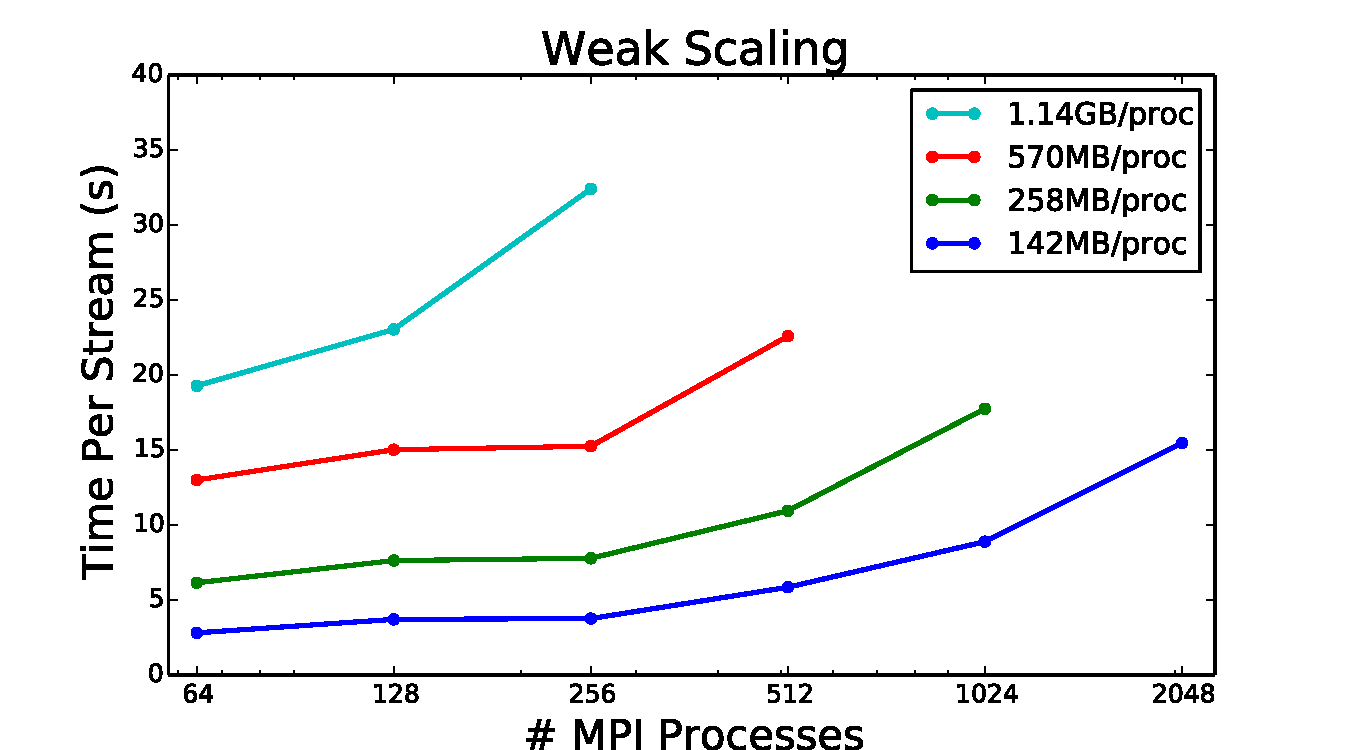
\includegraphics[width=0.9\columnwidth]{figures/weak_scaling.pdf}
  \caption{Per-stream times of \ourmethod in a weak-scaling experiment. }
  \label{fig:kronspeed_weak}
\end{figure}

\subsubsection{Strong Scaling}
In strong-scaling, the size of the data is fixed while the number of processes inreases. 
Strong-scaling is heavily penalized by serial portions of code (as dictated by Amdahl's law). \ourmethod exhibits a high degree of parallelism, illustrated in~\RefFigure{fig:kronspeed_strong}. 

\begin{figure}[b!]
\centering
  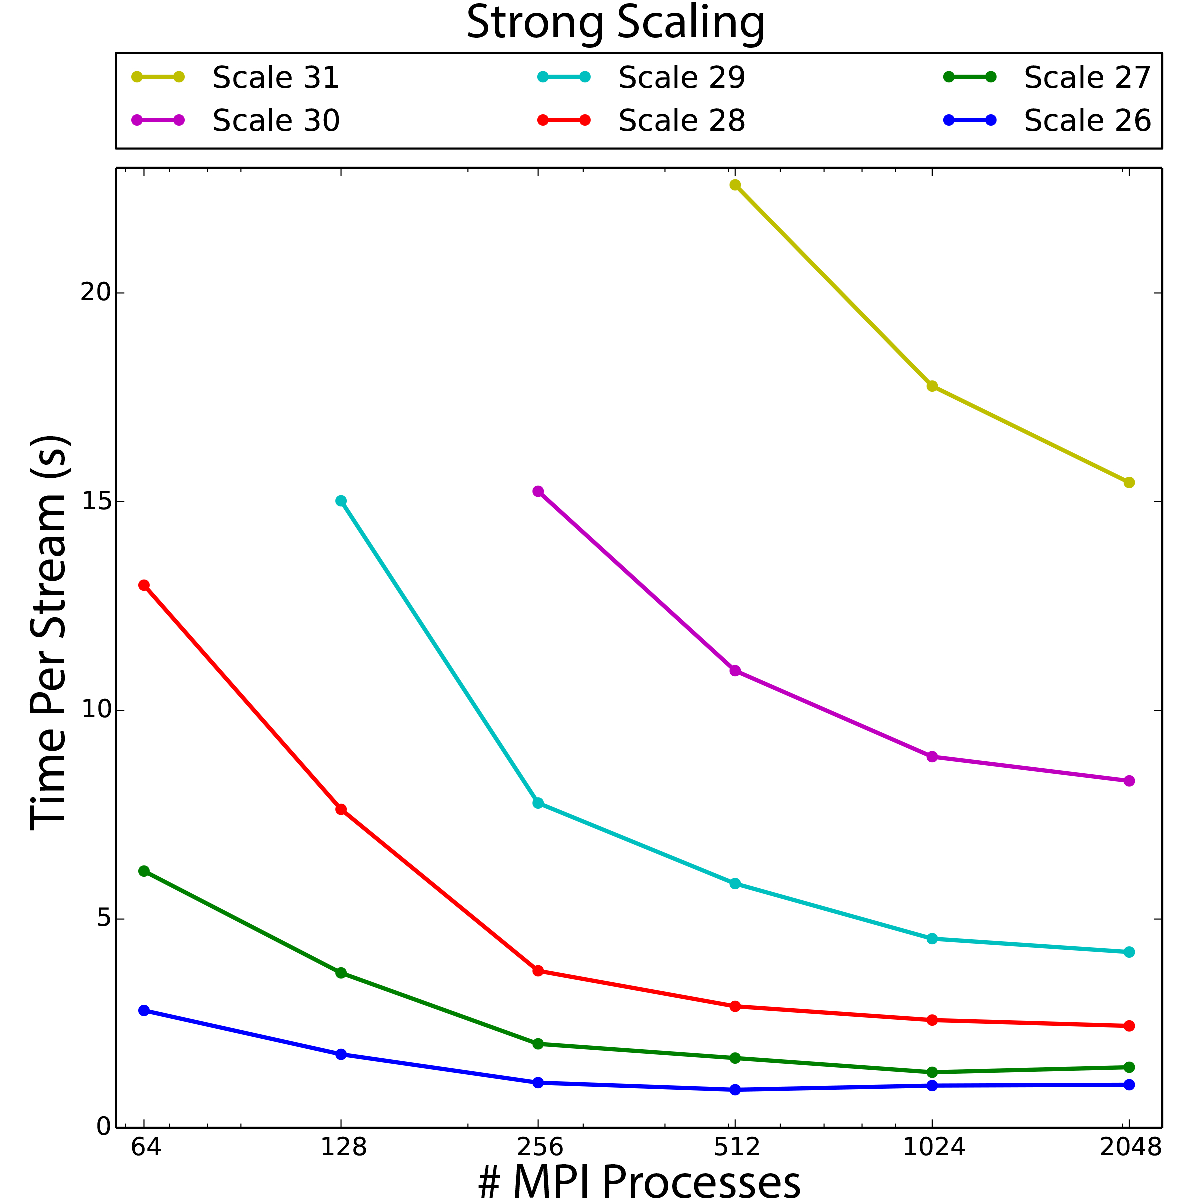
\includegraphics[width=0.9\columnwidth]{figures/strong_scaling.pdf}
  \caption{Per-stream times of \ourmethod for various strong-scaling data sizes. For instance, we can perform a single partitioning pass over a 34 billion edge, 2.1 billion node network in just 15 seconds.}
  \label{fig:kronspeed_strong}
\end{figure}

\subsection{Quality}
In \RefTable{table:big} we show some properties of our real test-graphs, as well as the performance of our streaming partitioner on them, for $k=2$ and $k=8$. We also compare our partition quality with ParMETIS.
In~\RefFigure{fig:kronqual}, \ourmethod performs comparably with parMETIS. Streaming partitioning is a valid alternative to conventional offline approaches and can be integrated in distributed-memory, on-the-fly algorithms for big-data.

\begin{figure}[h!]
\centering
  
\includegraphics[width=0.8\columnwidth]{figures/kronecker_quality_tests.pdf}
  \caption{Partition quality of various Kronecker graphs using \ourmethod compared to ParMETIS. We achieve comparable edges cut.}
  \label{fig:kronqual}
\end{figure}

\begin{figure}[t!]
\centering
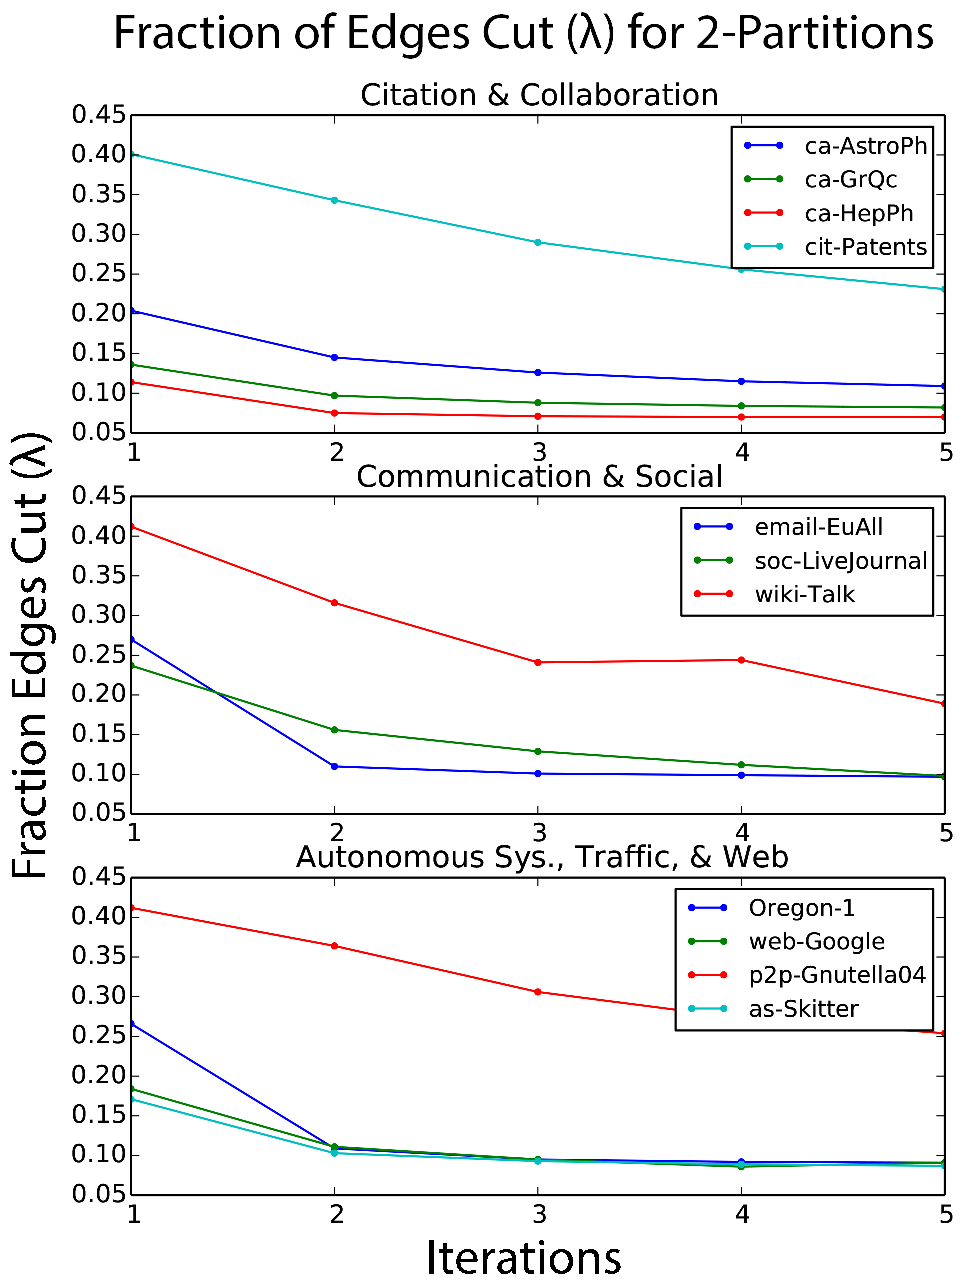
\includegraphics[width=0.9\columnwidth] {figures/real_k2_lambda.pdf}
\caption[Caption for]{Improvement in the edges cut ($\lambda$) over 5 passes for bi-partitions of each graph. Because there are only two partitions, the algorithm is able to quickly fix mistakes it made in the initial partitioning. Many of the errors made in the first pass are fixed in the second iteration, with diminishing improvement thereafter.}
\label{fig:k2_lambda}
\end{figure}

\begin{figure}[t!]
\centering
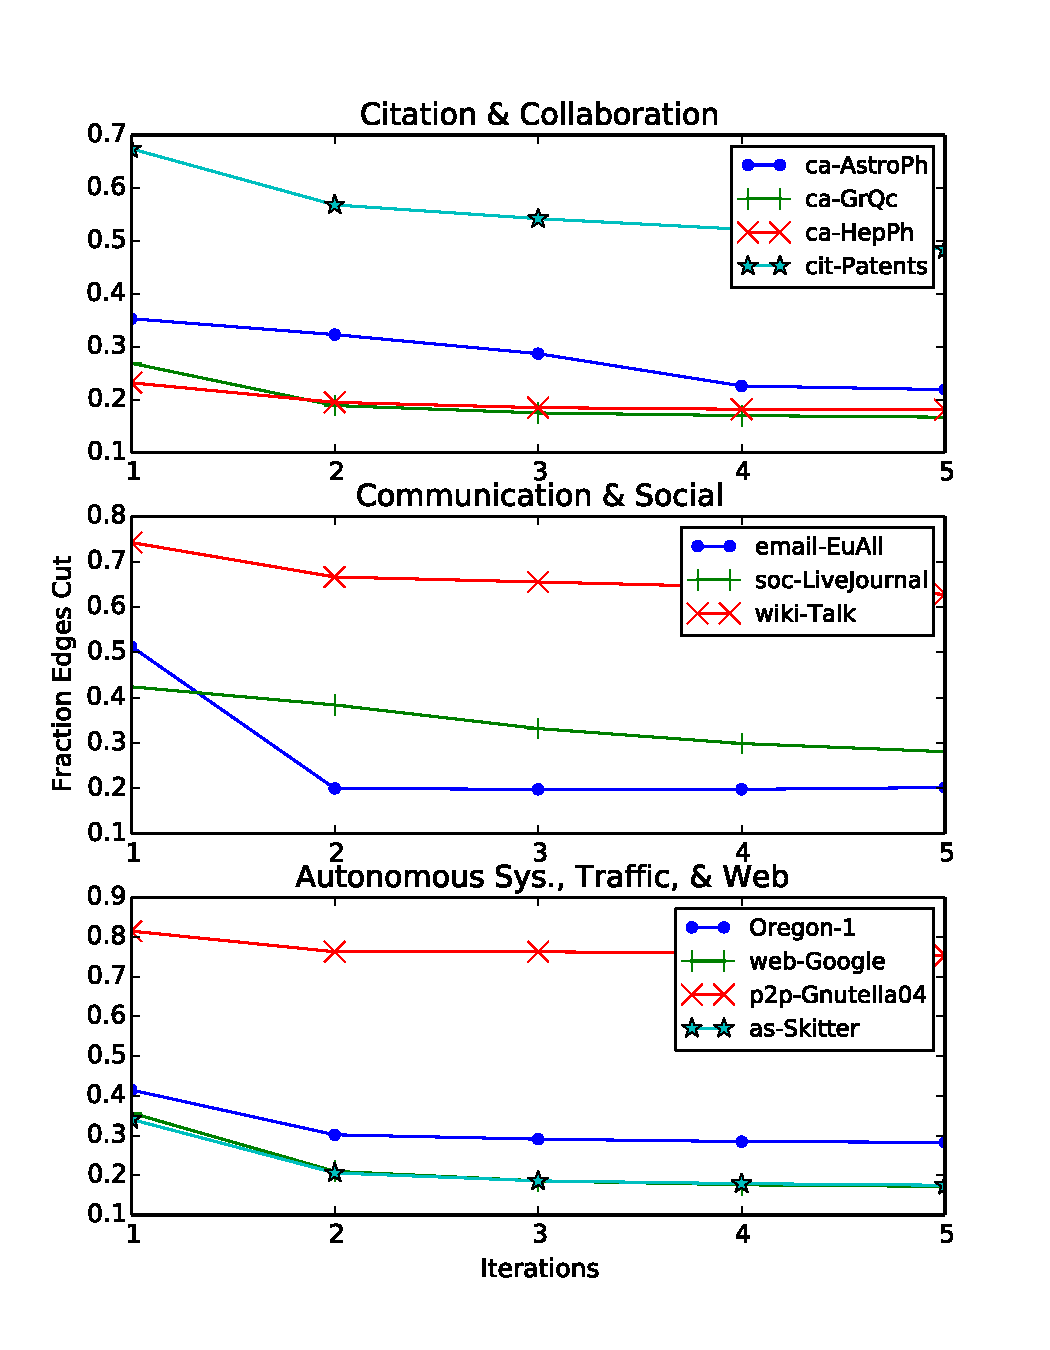
\includegraphics[width=0.9\columnwidth] {figures/real_k16_lambda.pdf}
\caption[Caption for]{Improvement in edges cut ($\lambda$) over 5 passes for $k=16$-partitions of each graph. Dividing the graph into 16 partitions makes the minimum edge cut problem much more challenging. Similar to the bi-partition results, we experience the best gain in the second pass and less in subsequent passes.}
\label{fig:k16_lambda}
\end{figure}

\subsection{Analysis}
Our scalability tests have demonstrated that \ourmethod is highly parallel and performs quality partitions far faster than our comptetitors. A single stream over a 34 billion edge, 2.1 billion node network can be done in just 15 seconds.

% Other data from real-world was harder to analyze -- there are not enough wide differences between data sets' results to draw strong conclusions.
Despite the complexity of many of the real graphs, \ourmethod creates well-balanced partitions.
While Power-Law graphs are overwhelmingly considered to be difficult to partition~\cite{Abou-Rjeili:2006:MAP:1898953.1899055}, we have demonstrated that a very simple, fast, algorithm is capable of significantly reducing communication in their parallel computation. 
We also demonstrate in~\RefFigure{fig:k2_lambda} and \RefFigure{fig:k16_lambda} that additional passes can further reduce edges cut (by up to a factor of 3). 

% Isolated comparisons we have made to the state-of-the-art partitioner METIS show that these results are competitive (usually within a factor of 2).
\REM{
One set of outlying (poorly-performing) data points are the Gnutella networks.
While Gnutella networks exhibit power-law-like topologies, elements of their algorithm truncate nodes from ever becoming extremely large. 
This heavy-clipping sets the Gnutella networks apart from many of the other social network topologies in our experiments.
The data set also has extremely low clustering coefficients and a very small number of closed triangles \cite{Ripeanu:2002:MGN:613352.613670}. 
Low clustering coefficients decrease the chance that neighbors of the current node-under-consideration share a partition. 
With more neighbors distributed across the partitions, many partitions will have roughly the same score, making optimal partition choices much harder.

A danger of naively running multiple passes is that one partition often becomes populated by very high-degree vertices. 
We attribute this to the ``dense core'' surrounded by a less-dense periphery that many scale-free graphs possess.
This can be observed qualitatively when scale-free graphs are embedded in a spectral space~\cite{Lang04findinggood}.

This dense partition tends to strongly emerge as we continue to make further passes of the streaming algorithm.
In order to overcome this we used the tempered parameter technique described in our methodology section. 
}
